\documentclass[12pt]{article}
\usepackage{settings}
\newcommand{\thesisLanguage}{deutsch} % 'english' or 'deutsch'
\newcommand{\student}{Max Mustermann}
\newcommand{\location}{Musterstadt}
\newcommand{\matrikelnumber}{777777}
\newcommand{\thesistitle}{This Is Your Thesis Title}
\newcommand{\thesistype}{Master's Thesis}
\newcommand{\course}{Applied Computer Science}
\newcommand{\faculty}{Computer Science and Engineering}
\newcommand{\hsname}{Esslingen University}

\newcommand{\period}{01.03.2024 - 31.08.2024}
\newcommand{\reviewer}{Prof. Dr. John Doe}
\newcommand{\secondReviewer}{Prof. Dr. Jane Doe}

% If you don't need a company, just leave the paranthesis empty: {}
\newcommand{\company}{Musterfirma GmbH}
\newcommand{\supervisor}{Albert Einstein}

\newcommand{\hslogo}{images/logos/HS-Logo-1.png}
% If you don't need a company logo, just leave the paranthesis empty: {}
\newcommand{\companylogo}{images/logos/mbti-logo-1.png}

% Define if ToDos should be displayed
\showtodostrue
%\showtodosfalse


% !!! DO NOT CHANGE THIS
\newcommand{\HRule}[2]{\noindent\rule[#1]{\linewidth}{#2}} % Horiz. Linie
\newcommand{\vlinespace}[1]{\vspace*{#1\baselineskip}} % Abstand
\newcommand{\titleemph}[1]{\textbf{#1}} % Hervorheben


% set date to null to hide it in the middle of the titlepage
\date{}

% include acronyms
\acsetup{make-links} % make acronyms clickable in text
\DeclareAcronym{API}{
    short = API,
    long = Application Programming Interface,
}

\DeclareAcronym{REST}{
    short = REST,
    long = Representational State Transfer,
}

\DeclareAcronym{JSON}{
    short = JSON,
    long =  JavaScript Object Notation,
}


% !!! IMPORTANT: COMPILE SPECIFIC CHAPTERS ONLY !!!
% \includeonly{content/01_Methodology}


\begin{document}
\author{}

\pagenumbering{gobble}

%make sure code listings are numbered by secions like in LoF
\counterwithin{lstlisting}{section}


% !!! IMPORTANT: REMOVE THIS LINE IF THE COVERPAGE IS NOT NEEDED !!!
\begin{titlepage}
    \centering
    \Large
    \vlinespace{4}
    \huge
    \textbf{\thesistitle} \\
    \vlinespace{4}

    \Large
    \thesistype \\
    \ifthenelse{\equal{\thesisLanguage}{english}}{%
        by\\
    }{%
        von\\
    }
    \Large
    \student
    \vlinespace{7}
    \ifthenelse{\equal{\thesisLanguage}{english}}{%

        Course of Studies: \course \\
        Faculty: \faculty\\
    }{%

        Studiengang: \course \\
        Fakultät: \faculty\\
    }
    \hsname\\

    %\vlinespace{2}

    \vfill

\end{titlepage}

% include titlepage
\begin{titlepage}
    \ifthenelse{\equal{\companylogo}{}}{%
        \hfill \includegraphics[height=1.3cm]{\hslogo}
    }{
        \includegraphics[height=1.3cm]{\companylogo} \hfill \includegraphics[height=1.3cm]{\hslogo}
    }
    \centering
    \Large
    \vfill
    \huge
    \vlinespace{2}
    \textbf{\thesistitle} \\
    \vlinespace{2}
    \Large
    \thesistype \\
    \ifthenelse{\equal{\thesisLanguage}{english}}{%
        by\\
    }{%
        von\\
    }
    \Large
    \student
    \vlinespace{3}

    \vlinespace{2}
    \ifthenelse{\equal{\thesisLanguage}{english}}{%
        Course of Studies: \course \\
        Faculty: \faculty\\
    }{%
        Studiengang: \course \\
        Fakultät: \faculty\\
    }
    \hsname\\

    \vlinespace{4}

    \vfill
    \raggedright
    \large
    \ifthenelse{\equal{\thesisLanguage}{english}}{%
        \titleemph{Period:} \period \\
        \titleemph{Reviewer:} \reviewer \\
        \titleemph{Second Reviewer:} \secondReviewer \\
    }{%
        \titleemph{Zeitraum:} \period \\
        \titleemph{Erstprüfer:} \reviewer \\
        \titleemph{Zweitprüfer:} \secondReviewer \\
    }


    % Folgenden Abschnitt nur bei Industrie-Arbeiten darstellen
    \ifthenelse{\equal{\company}{}}{%
        % \HRule{13pt}{1pt}
    }{%
        % If \company is not empty, check thesis language
        \vlinespace{1}
        \HRule{13pt}{1pt} \\
        \ifthenelse{\equal{\thesisLanguage}{english}}{%
            \titleemph{Company:} \company \\
            \titleemph{Supervisor:} \supervisor
        }{%
            \titleemph{Firma:} \company \\
            \titleemph{Betreuer:} \supervisor
        }
    }

\end{titlepage}

\onehalfspacing

\pagestyle{fancy}
\fancyhf{}
\fancyfoot[R]{\thepage}
\renewcommand{\headrulewidth}{0pt}


% !!! IMPORTANT: LOAD HERE YOUR STRUCTURE-CONTENT !!!
\ifthenelse{\equal{\thesisLanguage}{english}}{%
    \phantomsection\section*{Confidentiality Clause}
}{%
    \phantomsection\section*{Vertraulichkeitsklausel}
}

\ifthenelse{\equal{\thesisLanguage}{english}}{%
    By request of the company \company, the contents of this thesis — including any related data or drawings — are subject to confidentiality up to and including <<Month/Year>>.
    No copies or transcripts may be created, digitally or manually.
    Exceptions to this clause require written permission by the company \company.
}{%
    Auf Wunsch der Firma Musterfirma GmbH unterliegt der Inhalt dieser Arbeit - einschließlich der dazugehörigen Daten und Zeichnungen - bis einschließlich „Monat/Jahr“ der Geheimhaltung.
    Es dürfen keine Kopien oder Abschriften erstellt werden, weder digital noch manuell.
    Ausnahmen von dieser Regelung bedürfen der schriftlichen Genehmigung der Firma Musterfirma GmbH.
}
\signature{\location}
\\\vspace{5ex}

\ifthenelse{\equal{\thesisLanguage}{english}}{%
    \noindent The prohibition on publishing this thesis is supported by:
}{%
    \noindent Das Verbot der Veröffentlichung dieser Arbeit wird unterstützt durch:
}
\\\vspace{5ex}

\noindent\begin{tabular}{lr}
    \reviewer, \today & \makebox[2.5in]{\hrulefill} \\
                      & \hspace{1pt}
    \ifthenelse{\equal{\thesisLanguage}{english}}{%
        Signature
    }{%
        Unterschrift
    }
\end{tabular}
\\\vspace{5ex}
\ifthenelse{\equal{\thesisLanguage}{english}}{%
    \phantomsection\section*{Declaration of Independent Work}
}{%
    \phantomsection\section*{Selbstständigkeitserklärung}
}

\ifthenelse{\equal{\thesisLanguage}{english}}{%
    I hereby declare that I completed this work independently and that I have used no aids other than those referenced.\newline
    The parts of the work, which include phrases or points taken from other sources, are clearly marked with the origin of the information.
    This also applies to diagrams, sketches, visual representations as well as for sources from the Internet.\newline
    I also declare that I have not submitted this work in any other testing procedure as an examination paper, nor will I in the future.
}{%
    Ich erkläre hiermit, dass ich diese Arbeit selbständig verfasst und keine anderen als die angegebenen Hilfsmittel benutzt habe.
    Die Teile der Arbeit, die aus anderen Quellen entnommene Sätze oder Stellen enthalten, sind deutlich mit der Herkunft der Informationen gekennzeichnet.
    Dies gilt auch für Diagramme, Skizzen, bildliche Darstellungen sowie für Quellen aus dem Internet.
    Ich erkläre ferner, dass ich diese Arbeit in keinem anderen Prüfungsverfahren als Prüfungsarbeit eingereicht habe und auch in Zukunft nicht einreichen werde.
}
\signature{\location}

\ifthenelse{\equal{\thesisLanguage}{english}}{%
    \phantomsection\section*{Acknowledgements}
}{%
    \phantomsection\section*{Danksagung}
}

I would like to express my deepest appreciation to my professor, \reviewer, for his invaluable patience, insightful feedback, and unwavering support throughout this thesis. His guidance has been instrumental in shaping this work.
I am also profoundly grateful to my supervisor, \supervisor, from \company.
His generous provision of knowledge and expertise has been crucial to the success of this research.
Here you can also thank your family and friends or your pet :)
\newline
Thank you all for your significant contributions to this journey.
\phantomsection\section*{Abstract} % "*" to disable numbering
Nenne die Zielsetzung, die Problemstellung und die Forschungsfragen. Wenn deiner Abschlussarbeit bestimmte Hypothesen zugrunde liegen, erwähne diese auch.
Zähle die wichtigsten Ergebnisse deiner Forschung auf und erkläre, zu welchem Fazit du gekommen bist.
Nenne die relevantesten Eckpunkte aus der fachlichen Diskussion und lege deine Empfehlungen dar.
Nimm keinen Bezug auf Literatur und verwende keine Zitate.
Verzichte auf jegliche subjektiven Bewertungen oder Rechtfertigungen.
Benutze keine Abkürzungen.
Zeitform: Präsens, vergangene Ereignisse im Perfekt oder Präteritum



% include TOC
\microtypesetup{protrusion=false}
\newpage
\ifthenelse{\equal{\thesisLanguage}{english}}{%
    \renewcommand{\contentsname}{Contents}
}{%
    \renewcommand{\contentsname}{Inhaltsverzeichnis}
}
\tableofcontents
\thispagestyle{fancy}
\fancyhf{}
\fancyfoot[R]{\thepage}
\renewcommand{\headrulewidth}{0pt}
\microtypesetup{protrusion=true}


% include list of figures
\newpage
\pagenumbering{Roman}
\ifthenelse{\equal{\thesisLanguage}{english}}{%
    \phantomsection\addcontentsline{toc}{section}{List of Figures}
    \renewcommand{\listfigurename}{List of Figures}
}{%
    \phantomsection\addcontentsline{toc}{section}{Abbildungsverzeichnis}
    \renewcommand{\listfigurename}{Abbildungsverzeichnis}
}
\listoffigures
\thispagestyle{fancy}
\fancyhf{}
\fancyfoot[R]{\thepage}
\renewcommand{\headrulewidth}{0pt}


% include list of tables
\newpage
\ifthenelse{\equal{\thesisLanguage}{english}}{%
    \phantomsection\addcontentsline{toc}{section}{List of Tables}
    \renewcommand{\listtablename}{List of Tables}
}{%
    \phantomsection\addcontentsline{toc}{section}{Tabellenverzeichnis}
    \renewcommand{\listtablename}{Tabellenverzeichnis}
}
\listoftables
\thispagestyle{fancy}
\fancyhf{}
\fancyfoot[R]{\thepage}
\renewcommand{\headrulewidth}{0pt}


% include Code listings
\ifthenelse{\equal{\thesisLanguage}{english}}{%
    \renewcommand\lstlistingname{Listing}
    \renewcommand\lstlistlistingname{List of Listings}
}{%
    \renewcommand\lstlistingname{Quellcode}
    \renewcommand\lstlistlistingname{Quellcodeverzeichnis}
}
\newpage
\ifthenelse{\equal{\thesisLanguage}{english}}{%
    \phantomsection\addcontentsline{toc}{section}{List of Listings}
    \lstlistoflistings
}{%
    \phantomsection\addcontentsline{toc}{section}{Quellcodeverzeichnis}
    \lstlistoflistings
}


\thispagestyle{fancy}
\fancyhf{}
\fancyfoot[R]{\thepage}
\renewcommand{\headrulewidth}{0pt}


% include acronyms
\newpage
\ifthenelse{\equal{\thesisLanguage}{english}}{%
    \phantomsection\addcontentsline{toc}{section}{List of Abbreviations}
    \printacronyms[name=List of Abbreviations, template=supertabular]
}{%
    \phantomsection\addcontentsline{toc}{section}{Abkürzungsverzeichnis}
    \printacronyms[name=Abkürzungsverzeichnis, template=supertabular]
}


% include todos
\ifshowtodos
    \newpage
    \phantomsection\addcontentsline{toc}{section}{List of Todos}
    \listoftodos
    \thispagestyle{fancy}
    \fancyhf{}
    \fancyfoot[R]{\thepage}
    \renewcommand{\headrulewidth}{0pt}
\fi


% set pagestyle for normal textpages
\clearpage
\pagestyle{fancy}
\fancyhf{}
\fancyhead[L]{\leftmark}
%\fancyhead[R]{\rightmark}
\fancyfoot[R]{\thepage}
\renewcommand{\headrulewidth}{1pt}
\pagenumbering{arabic}



% !!! IMPORTANT: LOAD HERE YOUR STRUCTURE-CONTENT !!!
\section{Generelles zu Abschlussarbeiten}
\subsection{Unterschiede zwischen Deutsch- und Englischer Abschlussarbeit}
Generell unterscheidet sich das Schreiben auf Englisch nicht groß vom Schreiben auf Deutsch. Allerdings gibt es ein paar Feinheiten, deren du dir bewusst sein solltest, wenn du mit dem Schreiben einer Arbeit auf Englisch beginnst.
\begin{table}[H]
    \centering
    \begin{tblr}{
            width = \linewidth,
            hlines,
            vlines,
        }
        \textbf{Deutsch}              & \textbf{Englisch}     \\
        Nominalstil                   & Reich an Verben       \\
        Sprache oft im Passiv         & Sprache im Aktiv      \\
        Oft langer, komplexer Satzbau & Kurze, einfache Sätze \\
    \end{tblr}
    \caption{Unterschiede zwischen Deutsch und Englischer Abschlussarbeit}
    \label{Unterschiede zwischen Deutsch und Englischer Abschlussarbeit}
\end{table}\noindent
Du solltest dir beim Schreiben deiner Arbeit darüber im Klaren sein, ob du in britischem oder auf amerikanischem Englisch schreibst.
Die Unterschiede sind groß und Einheitlichkeit ist sehr wichtig für das Gesamtbild deiner Abschlussarbeit.
Dass Nomen im Englischen nicht großgeschrieben werden, solltest du wissen.
Aber es gibt noch mehr Unterschiede im akademischen Englisch, so werden zum Beispiel, je nachdem welches Format du nutzt, in Überschriften oft fast alle Wörter ‚capitalized‘.



\subsection{Aufbau einer Abschlussarbeit}
Generell solltest du dir zuerst die Ziele deiner Arbeit überlegen. Daraus entsteht dann die Zielsetzung.
Außerdem solltest du eine Literaturrecherche machen, um deine Arbeit in den Kontext anderer Arbeiten zu setzen und die Problemstellung klar herausarbeiten zu können. Dein Aufbau deiner Thesis kann verschieden sein, jedoch habe ich folgenden Aufbau benutzt:
\begin{itemize}
    \item Introduction / Einleitung
          \begin{itemize}
              \item Problem Statement / Problemstellung
              \item Objectives / Ziele dieser Arbeit
              \item Structure of this Thesis / Aufbau dieser Arbeit
              \item Related Work / Verwandte Arbeiten
          \end{itemize}
    \item Fundamentals / Grundlagen
          \begin{itemize}
              \item Hier erklärst du grundlegende Technologien oder Begriffe, die für das Verständnis deiner Arbeit relevant sind
          \end{itemize}
    \item ... Der weitere Aufbau hängt stark davon ab, ob du etwas praktisches machst etc. Oft gliedert man in Design und Implementierung.
    \item Summary and Outlook / Zusammenfassung und Ausblick
          \begin{itemize}
              \item Results / Ergebnisse
              \item Discussion / Diskussion
              \item Conclusion / Fazit
              \item Future Work / Ausblick
          \end{itemize}
\end{itemize}
\section{Wie benutzt man diese Vorlage}
\subsection{Konfiguration und Generelles}
Diese Vorlage ist so aufgebaut, dass du nichts mehr konfigurieren oder einstellen musst.
Stattdessen kannst du dich auf das Schreiben deiner Arbeit konzentrieren.
Im Hauptverzeichnis liegt die Datei \verb|01_config.tex|.
In dieser Datei werden die Grunddaten deiner Arbeit festgelegt.
Dazu zählt auch die Sprache.
Hier kannst du entscheiden, ob du deine Arbeit auf Deutsch oder Englisch verfassen möchtest.
Je nachdem welche Sprache du verwendest, werden alle Inhalte automatisch in der entsprechenden Sprache dargestellt (außer natürlich dein geschriebener Text).
Außerdem legst du in dieser Datei dein Name, Titel, Prüfer und alles weitere fest.
Dies dient dazu, damit diese an entsprechender Stelle automatisch geladen werden können.
Möchtest du also zum Beispiel in deiner Danksagung den Erstprüfer erwähnen, so musst du nur den Befehl \verb|\reviewer| benutzen.

Außerdem empfehle ich, deinen Text sinnvoll in Dateien zu gliedern.
Du kannst zum Beispiel jedes Kapitel in eine Datei packen.
Ein Beispiel ist hier schon gegeben.
Über die Datei \verb|main.tex| werden dann deine Dateien eingebunden (siehe Zeile 154).
Um die Compile-Zeit zu steigern, kannst du auch nur einzelne Dateien laden.
Dies passiert in Zeile 12 in \verb|main.tex|.
Hier gibst du die Dateien an, an welchen du aktuell arbeitest.
Der Vorteil hierbei ist, dass Referenzen auf andere Kapitel oder Bilder aus anderen Kapitel dennoch dargestellt werden können, und keine Compile-Fehler auftreten.

Standardmäßig enthält die generierte PDF eine Coverseite.
Diese kannst du beim Drucken gut als erste Seite oder als Cover benutzen.
Brauchst du diese Seite nicht, kannst du Zeile 26 in \verb|main.tex| auskommentieren oder löschen.



\subsection{Nummerierung von Bilder, Tabellen etc.}
Bilder, Tabellen etc. werden automatisch nummeriert.
Was jedoch kurz für Verwirrung sorgen kann, ist die Art und Weise der Nummerierung.
Alle Elemente besitzen die erste Zahl entsprechend des Kapitels, in dem sie sich befinden.
Sprich, Abbildung 3.5 befindet sich in Kapitel 3.
Die zweite Zahl wird beginnend bei 1 und fortlaufend generiert.
Diese Art der Nummerierung wird häufig bei Abschlussarbeiten verwendet.



\subsection{Overleaf oder andere IDEA?}
Generell empfehle ich dir, jeden Satz in einer neuen Zeile im Editor zu beginnen.
Dies erleichert die Lesbarkeit deines Codes und ermöglicht, falls du mit der Overleaf Review Funktion arbeitest oder mit Git, bessere Kommentare durch deinen Betreuer.
Aufgrund der doch langen Compile-Zeit von Overleaf bei größeren Arbeiten empfehle ich die Verwendung von TexLive und Visual Studio Code für Windows (\href{https://blog.jakelee.co.uk/getting-latex-working-in-vscode-on-windows/}{Hier eine Anleitung}).
Über Git kannst du deine Arbeit sichern und dein Betreuer kann z.B. über Issues Anmerkungen machen.
Wenn du mit Visual Studio Code arbeitest und deine Sätze sehr lang sind, kannst du horizontales Scrollen vermeiden über \verb|View| $\rightarrow$ \verb|Word Wrap|



\subsection{Abkürzungen verwenden}
In der Datei \verb|02_abbreviations.tex| musst du deine Abkürzungen festlegen.
Einige Beispiele sind bereis in der Datei enthalten.
Möchtest du eine Abkürzung verwenden, benutze einfach den Befehl \verb|\ac{...}|.
Um die Plural-Form zu verwenden, benutze den Befehl \verb|\acp{...}|.
LaTeX erkennt automatisch, wenn du die Abkürzung das erste Mal verwendest und schreibt diese aus.
Außerdem werden im Abkürzungsverzeichnis nur die Abkürzungen dargestellt, die du auch verwendest.
Es ist also nicht schlimm, eine zu lange \verb|02_abbreviations.tex|-Datei zu haben.
Das Abkürzungsverzeichnis ist außerdem bereits automatisch alphabetisch sortiert.
Ansonsten passiert alles automatisch - außer die beiden Befehle benutzen brauchst du nichts weiter tun.
So sieht dann eine verwendete Abkürzung aus: \ac{API}



\subsection{Quellenangaben verwenden}
In der Datei \verb|references.bib| werden deine Quelle festgelegt.
Auch hier sind einige Beispiele bereits in der Datei vorhanden.
Um eine Quelle in deinem Text zu benutzen, verwende den Befehl \verb|\cite{...}|.
Wie bereits bei den Abkürzungen werden alle verwendeten Quellen automatisch in das Literaturverzeichnis geladen.
Eine verwendete Quellenangabe sieht dann am Ende so aus im Text \cite{test}.
Wenn du möchtest, kannst du den Zitier-Style ändern.
Dies geschieht über Zeile 52 und 53 in der Datei \verb|settings.sty|.
Jedoch empfehle ich für Abschlussarbeiten an der Fakultät IT die bereits hinterlegte numerische Zitierweise.

Zum organisieren deiner Quellen kann ich dir Zotero empfehlen.
Hier kannst du deine ganzen Quellen verwalten, sortieren, mit Tags versehen wie zum Beispiel "noch nicht gelesen", und vieles mehr.
Der Vorteil ist, dass du in Zotero die \verb|.bib|-Datei generieren lassen kannst und diese dann ganz einfach in deiner Thesis verwenden kannst.
Außerdem bietet Chrome eine Zotero-Erweiterung an.
Mit dieser können Paper, Artikel, Websiten etc. super schnell und unkompliziert als Quelle gespeichert werden, meist automatisch mit den richtigen Angaben wie Autoren, Datum, etc.
Außerdem werden in Zotero die PDFs gespeichert, heißt du musst beim nachlesen von Sachen in deinen Quellen nicht immer erst die PDF wieder im Netz suchen.



\subsection{Bilder einbinden}
Für Bilder ist bereits der Ordner \verb|/images| hinterlegt.
Speichere also alle Bilder dort.
Wenn möglich, vor allem bei Grafiken, sollte das PDF Format bevorzugt werden.
Dies ermöglicht eine scharfe Darstellung.
Um eigene Grafiken zu erstellen, empfehle ich dir \href{https://app.diagrams.net/}{app.diagrams.net/}.
Hier kannst du einfach und unkompliziert alles als PDF exportieren.
Falls du eine Grafik aus einer Quelle benutzt, empfehle ich dir, diese "nachzubauen" und anschließend einen Vermerk anzugeben mit Referent zum Original.

Das \verb|[b]| beschreibt, wie dein Bild floaten soll.
Generell wird empfohlen, auch bei den meisten Papern, dass Bilder entweder auf Seiten oben oder unten floaten sollen.
\verb|b| steht dabei für "bottom", also das Seitenende.
\verb|t| wird benutzt, um das Bild oben floaten zu lassen.
\verb|h| kannst du benutzen, um das Bild an genau dieser Stelle zu generieren.
Dies kann auch verwendet werden, falls es dein Erstprüfer erlaubt.
Generell gelten diese Floating-Optionen auch für Tabellen, Quellcode oder Pseudocode.

Zum Einbinden von Bildern, benutze den folgenden Code:
\begin{verbatim}
    \begin{figure}[b]
        \centering
        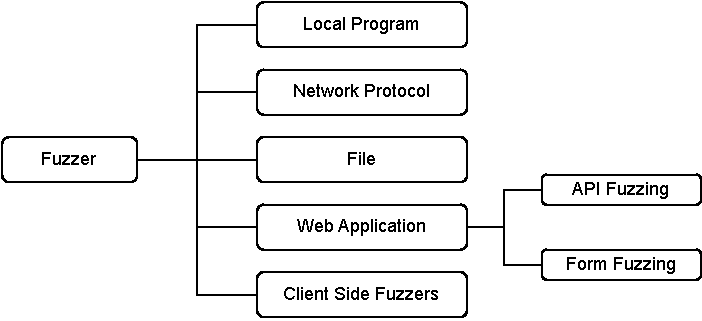
\includegraphics[width=0.85\textwidth]{example.pdf}
        \caption[Some Caption]{Some Caption (based on \cite{test})}
        \label{img:bla}
    \end{figure}
\end{verbatim}\noindent
Über \verb|width=0.85\textwidth| gibst du an, wie breit dein Bild sein soll.
Ich empfehle hier, einen Wert von 0.95 nicht zu überschreiten.

Über \verb|\caption| gibst du die Bildunterschrift an.
Falls du, wie zuvor erwähnt, auf eine Quelle verweisen möchtest, benutze die geschweiften Klammern.
Dies sorgt dafür, dass die Caption in den eckigen Klammern im Abbildungsverzeichnis dargestellt wird und die Caption in den geschweiften Klammern unter dem Bild selber.

Um auf das Bild verweisen zu können (wird in \autoref{sec:ref} erklärt), musst du den Befehl \verb|\label| benutzen und das Label definieren.
Dies wird anschließend benutzt, um das Bild zu refenzieren.
Hier kannst du dir ein Schema überlegen, zum Beispiel für Bilder "img:...".

Hier ist ein Beispiel, wie ein Bild mit der Floating-Option \verb|h| aussieht:
\begin{figure}[h]
    \centering
    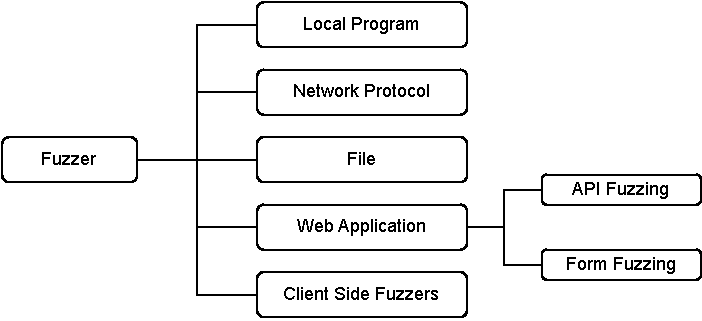
\includegraphics[width=0.75\textwidth]{example.pdf}
    \caption[Some Caption]{Some Caption (based on \cite{test})}
    \label{img:bla}
\end{figure}



\subsection{Tabellen einbinden}
Das Einbinden von Tabellen funktioniert prinzipiell genau gleich wie mit Bilder.
Es gibt die Floatin-Option, eine Caption sowie ein Label.
Auch hier kannst du optional für die Caption eckige Klammern benutzen.
Hier ist ein Beispiel für eine Tabelle.
Schaue dir einfach den Code an, dieser ist selbsterklärend.
\begin{table}[h]
    \centering
    \begin{tblr}{
            width = \linewidth,
            hlines,
            vlines,
        }
        \textbf{Fuzzer} & \textbf{Test 2}     \\
        APIFuzzer       & \color{red}failed   \\
        OFFAT           & \color{red}failed   \\
        openapi-fuzzer  & \color{red}failed   \\
        RESTler         & \color{red}failed   \\
        RestTestGen     & \color{green}passed \\
    \end{tblr}
    \caption{Some Caption}
    \label{tbl:bla}
\end{table}\noindent



\subsection{Quellcode einbinden}
Für das Einbinden von Quellcode wird das Verzeichnis \verb|\code| benutzt.
Hier legst du einfach deine Quellcodedatien ab, welche du darstellen möchhtest.
Quellcode bindest du über den folgenden Befehl ein:
\begin{verbatim}
    \lstinputlisting[float=b, caption=Some Caption, label=lst:bla]{redos.ts}
\end{verbatim}\noindent
Auch hier können die bereits beschriebenen Float-Optionen verwendet werden.
Aus Gründen der Übersichtlichkeit verzichtet meine Vorlage auf farbliches Hervorheben im Quellcode.
Generell solltest du nur die relevanten Zeilen im Quellcode darstellen, welche absolut relevant sind.
Die vollständige Datei kannst du dann zum Beispiel im Anhang einfügen.
Benutze hierfür die beispielhafte Datei \verb|/content/99_appendix.tex|
\lstinputlisting[float=h, caption=Some Caption, label=lst:bla]{redos.ts}



\subsection{Pseudocode einbinden}
Es kann vorkommen, dass du Pseudocode oder Algorithmen zum Beispiel im Rahmen eines Designs einbinden möchtest.
Hier siehst du ein Beispiel, wie ein Algorithmus eingebunden ist.
Schaue dir einfach den Code dazu an, dieser ist selbsterklärend.
Auch hier gibt es wieder die bekannten Elemente wie die Floating-Option, die Caption und das Label.
\begin{algorithm}[h]
    \caption{Handling basic authentication via configuration file}
    \label{pseudo:bla}
    \begin{algorithmic}[1]
        \Function{GetAuthData}{config}
        \State...
        \State \Return userID, password
        \EndFunction

        \Function{GenerateBasicAuthHeader}{userID, password}
        \State credentials $\leftarrow$ userID + `:' + password
        \State encodedCredentials $\leftarrow$ \Call{Base64Encode}{credentials}
        \State authHeader $\leftarrow$ `Authorization: Basic ' + encodedCredentials
        \State \Return authHeader
        \EndFunction

        \vspace{3pt}
        \State configFilePath $\leftarrow$ `path/to/config/file'
        \State userID, password $\leftarrow$ \Call{GetAuthData}{configFilePath}
        \State authHeader $\leftarrow$ \Call{GenerateBasicAuthHeader}{userID, password}
        \State ...
    \end{algorithmic}
\end{algorithm}


\subsection{Referenz zu Kapiteln, Bildern, Tabellen etc.}
\label{sec:ref}
Du solltest darauf achten, dass jedes Bild, jede Tabelle, jeder Quellcode etc. auch im Text erwähnt wird.
Dabei kannst du mit Hilfe des \verb|\autoref{...}| Befehls schnell und unkompliziert auf das Element verweisen.
Innerhalb der geschweiften Klammern schreibst du das Label, das du definiert hast.
Alle refenzierten Inhalte sind außerdem anklickbar.
Hier ein Beispiel:

Zu diesem Zweck fügen wir einen neuen Pfad \texttt{redos} hinzu, der mit der HTTP-Methode \texttt{GET} aufgerufen wird, wie in \autoref{lst:bla} dargestellt.



\subsection{ToDos}
In diese Vorlage ist die Verwendung von ToDos integriert.
Dies kann dir dabei helfen, deinen aktuellen Fortschritt besser zu verfolgen oder auch eine bessere Kommunikation mit deinem Betreuer ermöglichen.
Die folgenden ToDos stehen dabei zur Verfügung:
\begin{verbatim}
    \toDo{XY muss noch eingebaut werden}
    \improvement{Du könntest noch etwas genauer über AB schreiben}
    \approve
    \approved
\end{verbatim}\noindent
\toDo{XY muss noch eingebaut werden}
\improvement{Du könntest noch etwas genauer über AB schreiben}
\approve
\approved
Falls du dieses Feature nicht brauchst, kommentiere Zeile 26 in \verb|01_config.tex| ein und lösche Zeile 27.
Wenn du die ToDos verwendest und am Ende deine finale PDF generieren möchtest, brauchst du nicht alle ToDos manuell entfernen. Hierzu kannst du auch einfach Zeile 26 in \verb|01_config.tex| einkommentieren und Zeile 27 löschen.



% include bibliography
\newpage
\clearpage
\pagestyle{fancy}
\fancyhf{}
\fancyhead[L]{\leftmark}
\fancyfoot[R]{\thepage}
\renewcommand{\headrulewidth}{1pt}
\ifthenelse{\equal{\thesisLanguage}{english}}{%
    \phantomsection\printbibliography[heading=bibintoc]
}{%
    \phantomsection\printbibliography[heading=bibintoc, title={Literaturverzeichnis}]
}



% !!! IMPORTANT: INCLUDE YOUR APPENDIX HERE !!!
\appendix
\section{Anhang}
\label{Code Appendix}

\subsection{Script to Search for GitHub Repositories}
\label{Script to search for GitHub repositories}
\autoref{Python script so search for GitHub repositories} is used to search on GitHub for repositories matching the keywords provided by the user.
In comparison to a manual search, this script offers several advantages.
Firstly, the output includes all repositories found, and secondly, the output produces a link to the repository, which can then be used for further processing.
We developed this script by making use of the capabilities of ChatGPT 3.5, a sophisticated large language model \cite{openai_chatgpt_2024}.
\lstinputlisting[language=Python, caption=Python script so search for GitHub repositories, label=Python script so search for GitHub repositories]{git_search.py}


\newpage
\subsection{Script to Process Output Produced by RestTestGen}
\label{Script to process output produced by RestTestGen}
Since RestTestGen generates a \ac{JSON} file for every request sent, we need to search through these files to identify any errors found by RestTestGen.
To automate this process, we developed a Python script shown in \autoref{Python script to search inside RestTestGen output folder for found errors}.
The script takes two parameters: the directory containing the \ac{JSON} files and the search term to look for within these files.
To search for errors in the files, we use the search term "FAIL".
We developed this script by making use of the capabilities of ChatGPT 3.5, a sophisticated large language model \cite{openai_chatgpt_2024}.
\lstinputlisting[language=Python, caption=Python script to search inside RestTestGen output folder for found errors, label=Python script to search inside RestTestGen output folder for found errors]{string_search.py}


\end{document}